\chapter{Założenia projektowe \label{chap:zalozenia}}
Podczas realizacji postawionego zadania starano się zachować w jak największym stopniu realia rozgrywek \texttt{Robocup}, ze szczególnym uwzględnieniem zasad ligi \emph{Small-size League}.
Z racji, iż wczesniejsze prace prowadzono na symulatorze \emph{Player/Stage/Gazebo} zdecydowano się na dalsze prace na tej platformie.
Zachowano schemat przepływu informacji z pracy inżynierskiej. Został on zamieszczony na rysunku \ref{fig:przeplyw_sterowania}. Stosowany w rozgrywach \emph{Small-size League} został
zamodelowany jako osobna warstwa  aplikacji, komunikująca się bezpośrednio z symulatorem. Osobną warstwę stanowi także część aplikacji odpowiedzialna za sterowanie robotem.
\begin{figure}[H]
\centering
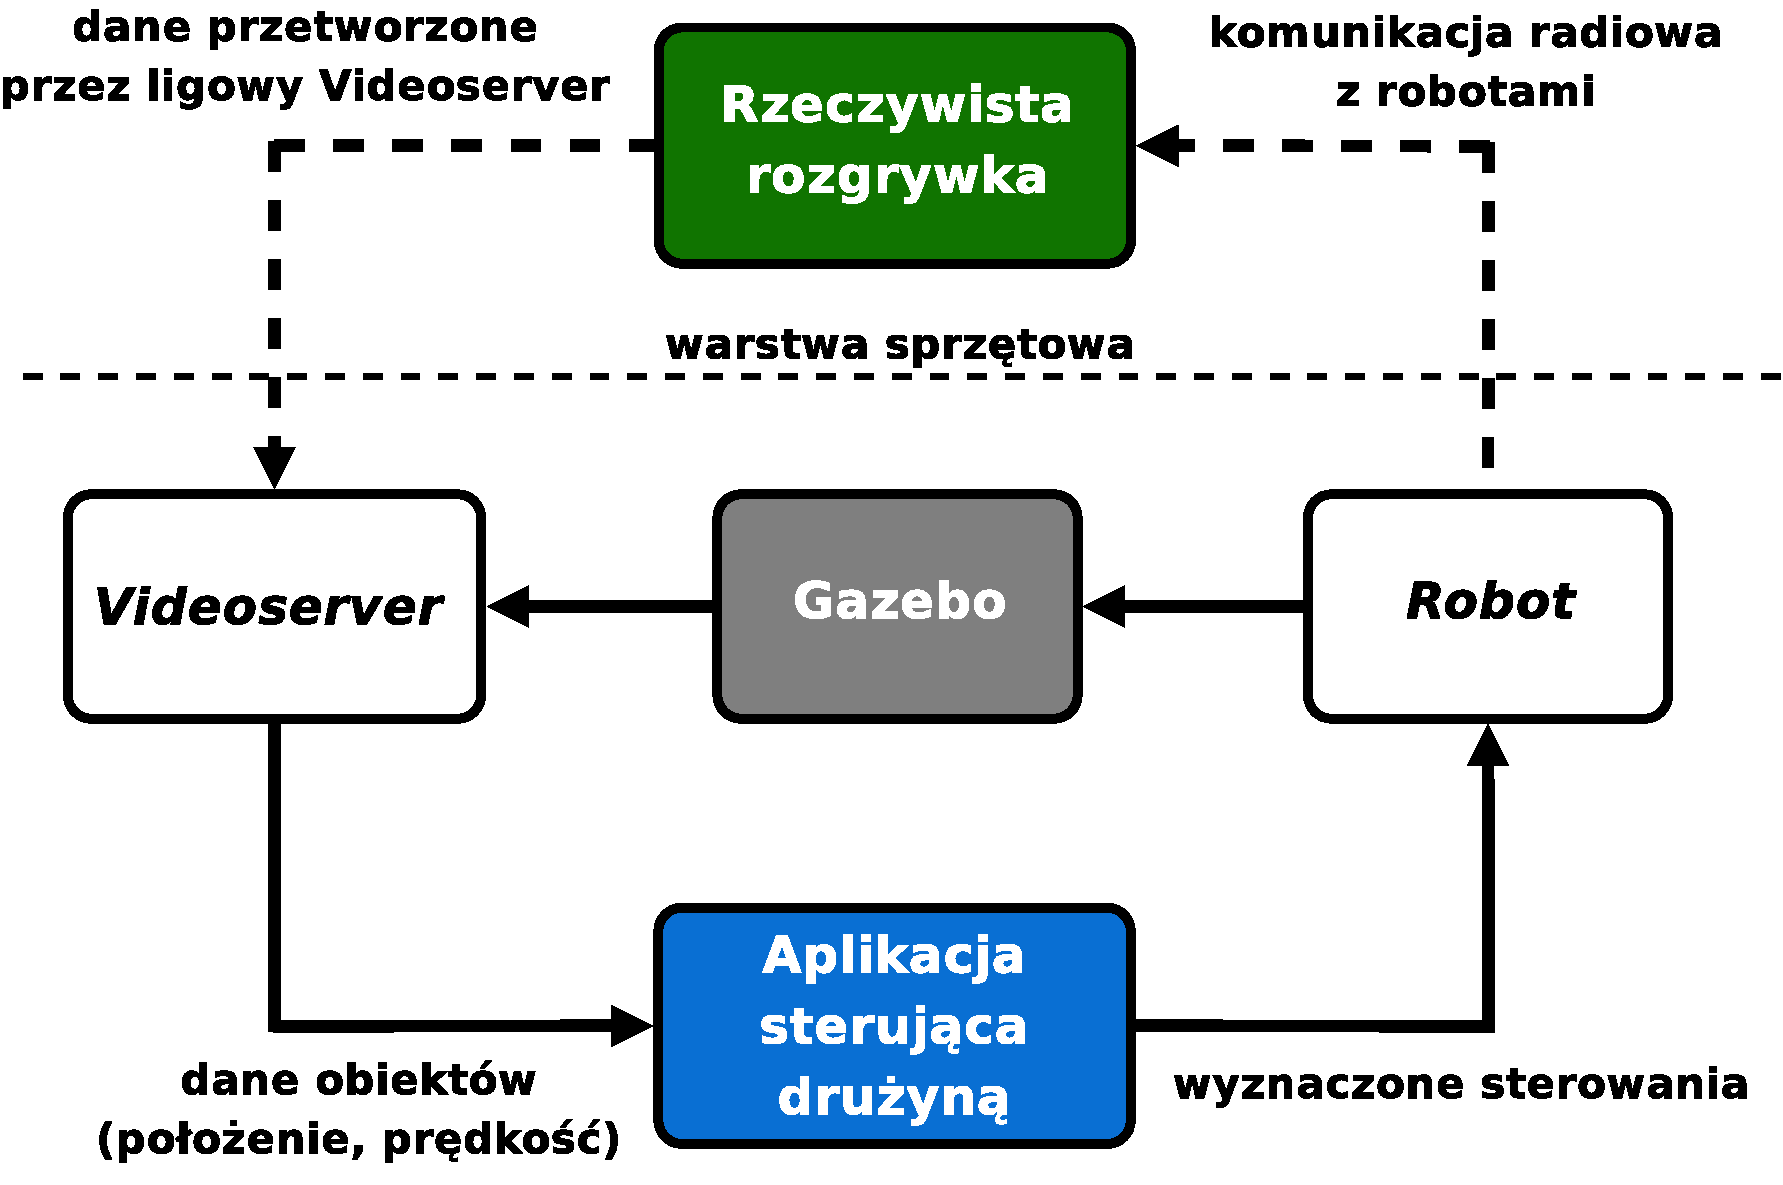
\includegraphics[scale=0.38]{./zalozenia/przeplyw_sterowania.pdf}
\caption{Komunikacja pomiędzy warstwami aplikacji.} \label{fig:przeplyw_sterowania}
\end{figure}
Dzięki takiej architekturze w łatwy sposób można przystosować aplikację do sterowania rzeczywistym robotem pobierającym dane z zewnętrznego serwera.
Zdecydowano się jednak na odejście od modelu robota o napędzie różnicowym. Tego typu baza jezdna wprowadza jednak znaczące ograniczenia na sterowanie takim zawodnikiem. W symulatorze zamodelowane zostały rzeczywiste
roboty biorące udział w rozgrywkach \emph{Small-size League}. Jak już wspomniano w rozdziale \ref{chap:robocup} są to roboty posiadające trzy niezależnie napędzane koła szwedzkie. Sterowanie takim zawodnikiem jest dużo
prostsze. Model został także wyposażony w urządzenie do dryblowania piłki oraz umożliwiające strzał lub podanie.
Przed przystąpieniem do prac nad architekturą aplikacji sterującej dokonano przeglądu rozwiązań stosowanych w rozgrywkach. Ostatecznie zdecydowano się na architekturę 
\mbox{\texttt{STP - Skill Tactics Play}} oryginalny opis można znaleźć w \cite{stp}. Natomiast w niniejszej pracy szerzej została ona omówiona w rozdziale \ref{chap:stp}.